\section{Experimental Results}
\label{s:experiments}
The section presents a representative sample of our experiments. The work \cite{Pro:26} contains a range of additional results.

\subsection{Data} \label{s:data}
In the experiment, we have selected 100 stocks with the highest average return in the year 2021, among the Fortune500 companies. Of those 100, we have further filtered out the 20 least pair-wise correlated among them. The experiment was conducted on more than 100 portfolios containing 8 to 12 randomly selected stocks out of those twenty. This was done mainly to reduce bias and have a methodological way to select the stocks for our portfolios.

The optimisation ran on market data from October 2022 to October 2025, which is about 750 trading days.  The first 125 days were used to collect $\bar{\mat{V}}_{\bar{t}}$ used to obtain the optimal prior $\mat{V}_0$, $\ref{s:prior}$. The following 125 trading days were to collect more data to run the structure estimation, $\ref{s:SE}$.

\subsection{Optional Parameters} \label{s:options}
The optional parameters primarily concern structure estimation and forgetting.

The parameters for our implementation of the genetic algorithm are: the batch size $=8$, $\text{p}_{\text{mut}} = 0.5$, and the decay rate for $\text{p}_{\text{mut}}$ was set at 0.992. The genetic algorithm ran for 500 iterations with each new portfolio.

The regressors in $\bar{x}_{t-1}$, among which the structure estimation selects significant ones, are the returns in the last 10 trading days, the difference between the long and short terms exponential moving averages, sine functions with differing periods, 10, 30 and 90 days and an intercept.

We made a $2^k$ experiment design \cite{4736103} to determine a good choice of remaining parameters, which are left to the user's responsibility. The data we used for this task were from 2021 to 2022. The model parameters from Secs, $\ref{s:prior}$, $\ref{s:forgetting}$ were set to $\alpha_0 = 0.09$, $\beta_0 = 0.5$, $\mu = 0.9$.

\subsection{Metrics and Base-Line Policies} \label{s:metrics}
The relevant metrics for portfolio optimisation reflect the primary goal of maximising returns and the secondary goal of low variance in those returns. The chosen metrics are: $\bullet$ maximum drawdown (the largest percentage loss experienced); $\bullet$ total return;
$\bullet$ average return;  $\bullet$ average return variance; and $\bullet$ Sharp ratio (SR$=
\mbox{average return}\,/\sqrt{\mbox{average return variance}}$.

Figures exploit the mean and median of these metrics evaluated across all the runs, cf.\ Sec.\ \ref{s:data}. Tables show the mean and median values of the considered metrics.

Our algorithm is called Risk-Averse and starts with uniform allocation. It considers $0.2\%$ cost for each transaction, which is low but common. Note that the majority of brokers offer fractional shares, so we don't have to care about that either.

Two types of portfolio choice serve us for comparison. The first, called Uniform Start, does not change the initial uniform allocation and therefore does not pay any transaction costs. The second, called Uniform, uniformly allocates funds to all assets. It is a theoretical ideal that is all the time perfectly diversified and does not consider transaction costs.

\subsection{Results and Discussion} \label{s:results}
The qualitative comparison provides figures. Plots \ref{fig:pareto_plotU}, \ref{fig:pareto_plotU-S}of average returns vs.\ average deviation of returns with indicated maximum drawdown compare our algorithm with both competitors. Each point reflects one portfolio.

Median of time evolutions of $\log(\mbox{SR})$ in Fig.\
 \ref{fig:sr_plot}, \ref{fig:sr_plotU-S} complements the qualitative picture.

 Tables show \ref{tab:metrics_mean}, \ref{tab:metrics_median} that our policy, despite paying transaction costs, behaves as the ideal Uniform policy that does not pay these costs. We are truly risk-averse as we improve maximum drawdown and consequently also total return. Compared to the Uniform Start policy, our improvements are even more visible.

\begin{figure}[H]
\centering
\begin{figure}[H]
    \begin{minipage}{0.45\textwidth}
    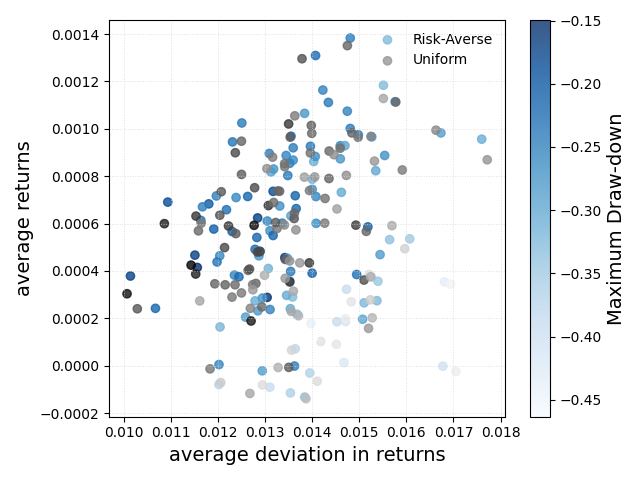
\includegraphics[width=\linewidth]{Images/ar_vs_ad_plot_HER_09mu.png}
    \caption{Average return vs. average deviation of returns for Risk Averse and and theoretically ideal Uniform portfolios.}
    \label{fig:pareto_plotU}
    \end{minipage}
    \vfill

    \begin{minipage}{0.45\textwidth}
    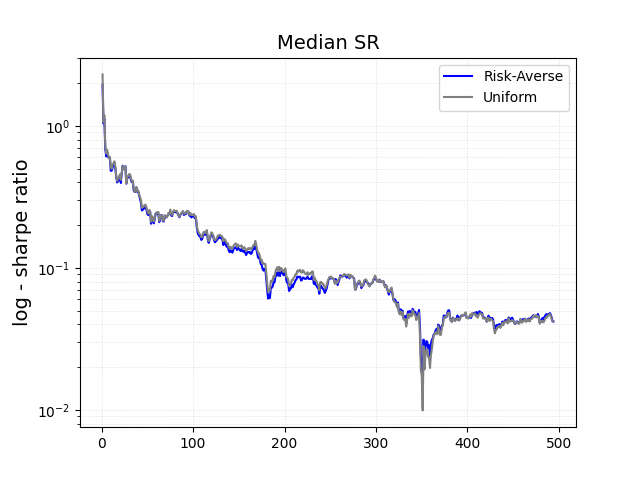
\includegraphics[width=\linewidth]{Images/mean_sr_HER_09mu.png}
    \caption{Sharpe ratio for Uniform \& Risk Averse portfolios.}
    \label{fig:sr_plot}
    \end{minipage}
\end{figure}

\begin{table}[H]
   \begin{minipage}{0.48\textwidth}
  % \centering
        \begin{tabular}{||l|r r||} % Example table
        \hline
        & Risk Averse & Uniform\\
        \hline
        max drawdown & -\textbf{0.273} & -0.280\\
        total return & 1.280 & 1.262 \\
        average return & 5.62e-4 & 5.37e-4 \\
        average return var. & 1.88e-4 & 1.86e-4 \\
        SR & 0.041 & 0.039 \\
        \hline
     \end{tabular}
  \end{minipage}
  \caption{Comparison of metrics' means $[\%]$}
          \label{tab:metrics_mean}
        \end{table}

  \begin{table}[H]
   \begin{minipage}{0.48\textwidth}
   % \centering
        \begin{tabular}{||l|r r||} % Example table
        \hline
        & Risk Averse & Uniform\\
        \hline
        max drawdown & -\textbf{0.259}& -0.271 \\
        total return & 1.269 & 1.265 \\
        average return & 5.68e-4 & 5.68e-4 \\
        average return var. & 1.84e-4 & 1.83e-4 \\
        SR & 0.042 & 0.042 \\
        \hline
        \end{tabular}
      \caption{Comparison of metrics' medians $[\%]$}
        \label{tab:metrics_median}
  \end{minipage}
\end{table}


\begin{figure}[H]
    \begin{minipage}{0.45\textwidth}
    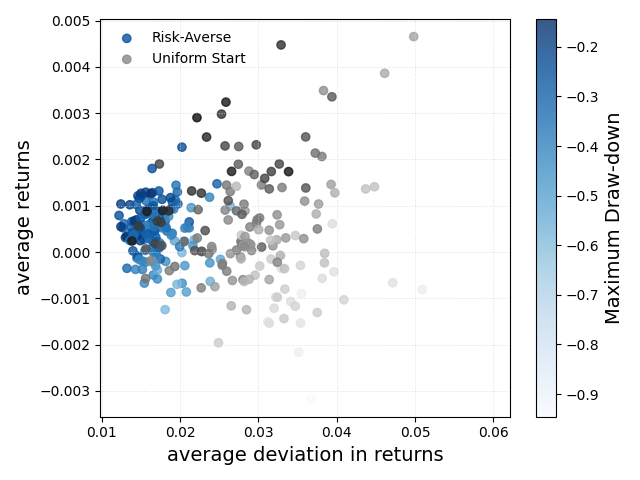
\includegraphics[width=\linewidth]{Images/ar_vs_ad_plot_HER_09_mu_se_uniformstart.png}
    \caption{Average return vs. average deviation of returns for Risk Averse and Uniform Start portfolios.}
    \label{fig:pareto_plotU-S}
    \end{minipage}
    \vfill

    \begin{minipage}{0.45\textwidth}
    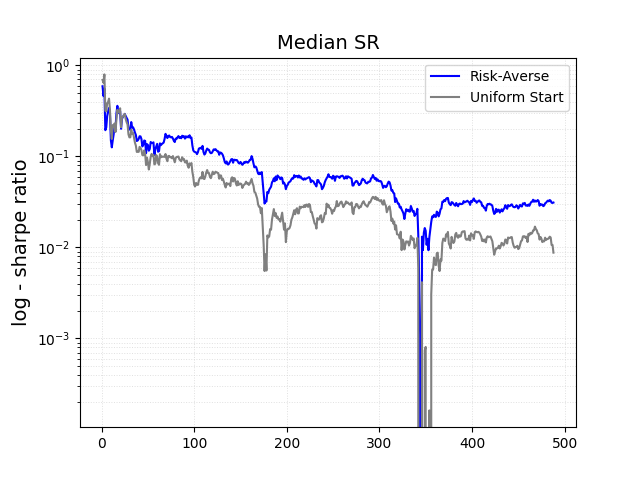
\includegraphics[width=\linewidth]{Images/median_sr_HER_09_mu_uniformstart.png}
    \caption{Sharpe ratio for Risk Averse \& Uniform Start portfolios.}
    \label{fig:sr_plotU-S}
    \end{minipage}
\end{figure}

\begin{table}[H]
    \begin{minipage}{0.48\textwidth}
        %\centering % Often good to center the table
        \begin{tabular}{||l|r r||} % Example table
        \hline
        & Risk Averse & Uniform Start\\
        \hline
        max drawdown & -\textbf{0.329} & -0.514\\
        total return & 1.21 & 1.222 \\
        average return & 4.58e-4 & 4.56e-4 \\
        average return var. & 2.94e-4 & 9.45e-4 \\
        SR & 0.027 & 0.015 \\
        \hline
        \end{tabular}
      \caption{Comparison of metrics' means $[\%]$} % <-- Use \captionof
        \label{tab:metrics_meanU-S}
    \end{minipage}
\end{table}

 \begin{table}[H]
    \begin{minipage}{0.48\textwidth}
      %  \centering % Often good to center the table
        \begin{tabular}{||l|r r||} % Example table
        \hline
        & Risk Averse & Uniform Start\\
        \hline
        max drawdown & -\textbf{0.316} & -0.499 \\
        total return & 1.18 & 0.915 \\
        average return & 5.17e-4 & 2.55e-4 \\
        average return var. & 2.75e-4 & 8.49e-4 \\
        SR & 0.031 & 0.009 \\
        \hline
        \end{tabular}
      \caption{Comparison of  metrics' medians $[\%]$}
        \label{tab:metrics_medianU-S}
    \end{minipage}
 \end{table}
 \end{figure} 